\chapter{Systems of Trust}
\label{sec:macroeconomics}

Bitcoin was not created in a vacuum and to understand the design of Bitcoin and by extension the Lightning Network one would
benefit from understanding money and systems of trust. Nakamoto encoded the string "the times 03/jan/2009 chancellor on brink of second bailout for banks"\cite{repository:bitcoin:sourceforge}\cite{bitcoin:genesis:coinbase} in the coinbase transaction of the genesis block as an alleged comment on the current banking system as well as a time stamp. He later cemented this view with multiple forum posts while he was still active\cite{nakamoto:post:deflation}\cite{nakamoto:govern:print}.

\section{Origin of money}

On the fringes of our specie barter became the first medium in which trade became viable, removing the risk from otherwise delayed reciprocity. It is possible for trade to be mutually beneficial as Nick Szabo so elegantly puts it:

\begin{displayquote}

"individuals, clans, and tribes all vary in their preferences, vary in their ability to satisfy these preferences, and vary in the beliefs they have about these skills and preferences and the objects that are consequent of them, there are always gains to be made from trade."\cite{szabo:shelling:out}

\end{displayquote}

Barter is by itself quite limited, consider a System \textbf{S}
consisting of \textbf{n} commodities, the amount of possible exchanges between commodities in \textbf{S} is \textbf{n x n}. When \textbf{n} eventually increases, the exchange pairs explodes exponentially. This makes it difficult to assess fair pricing and decreases the coincidence of a trade\footnote{The coincidence of finding another party who is looking to exchange the same commodity pair you are but in reverse order.}. The economist Carl Menger described it as inevitable for money to evolve from a sufficient volume of commodity barter\cite{menger:origins:money}. If the same System \textbf{S} is considered with money - the possible exchange pairs would be reduced to only \textbf{n} pairs. 

\subsection{Characteristics of money}
	\label{sec:characteristics:money}

Out of these commodities money emerged and history has provided many peculiar forms of money. The Rai stones of Yap islands, The Wampum shells in North America\footnote{The Wampum shells were actually legal tender as recently as 1710 in North Carolina and long into the 1600s in New England.}\cite{szabo:shelling:out} and Aggry beads in Africa to name a few. Although many different types of commodities have acted as money during certain time in history there are some characteristics that seem favorable and recur. The Federal Reserve Bank of Saint Louis lists them as\cite{fed:function:money}\footnote{Note that only the characteristics are from the Federal Reserve, the descriptions are not.}:

\begin{itemize}
	\item \textbf{Durability}. The ability to remain intact over time.
	
	\item \textbf{Portability}. The ability to move across physical distance.
	
	\item \textbf{Divisibility}. The ability to be divided across scale, to be used in any size of value transaction.
	
	\item \textbf{Uniformity}. The ability to use one unit interchangeably with another. Also referred to as \textbf{fungibility}.
	
	\item \textbf{Limited supply}. The ability to be scarce over time. Usually quantified by stock-to-flow. The amount of new supply in relation to already existing supply.
	
	\item \textbf{Acceptability}. The likelihood of being accepted in trade by others.
\end{itemize}

Many of the previous mentioned monies have expressed many of these characteristics well. Changes in these characteristics have also led to their downfall. Rai stones are carved limestone which are not native to the Yap islands, when outsiders started to bring in these on large ships it quickly changed their stock-to-flow ratio for the worst\cite{ammous:bitcoin:standard}. Aggry beads met the same fate when Europeans, with efficient means to produce them, started to export them to Africa and modernized shell fishing ruined the Wampum shells function as money\cite{szabo:shelling:out}.

Rare metals have held these attributes since the beginning of history and in many ways still hold them today. Gold especially stands out with it's very low stock-to-flow ratio.

\section{Bearer promissory notes}

Although gold emerged as the commodity best suited as money
it still had two major problems:

\begin{enumerate}
	\item Gold is unsuitable for small transactions due to the limit in divisibility.
	\item Gold is expensive to carry around and protect.
\end{enumerate}

Private and central banks began to issue bearer promissory notes to the owners of the underlying asset it stored(e.g figure \ref{fig:seb:promissory:note}). 
The asset could then be retrieved for the note on demand. The notes themselves could then be traded 
instead of the underlying gold. This solved both the above problems, notes are easy to carry, conceal and 
could be minted in very small amounts. 

\begin{figure}[!htb]

	\centering
	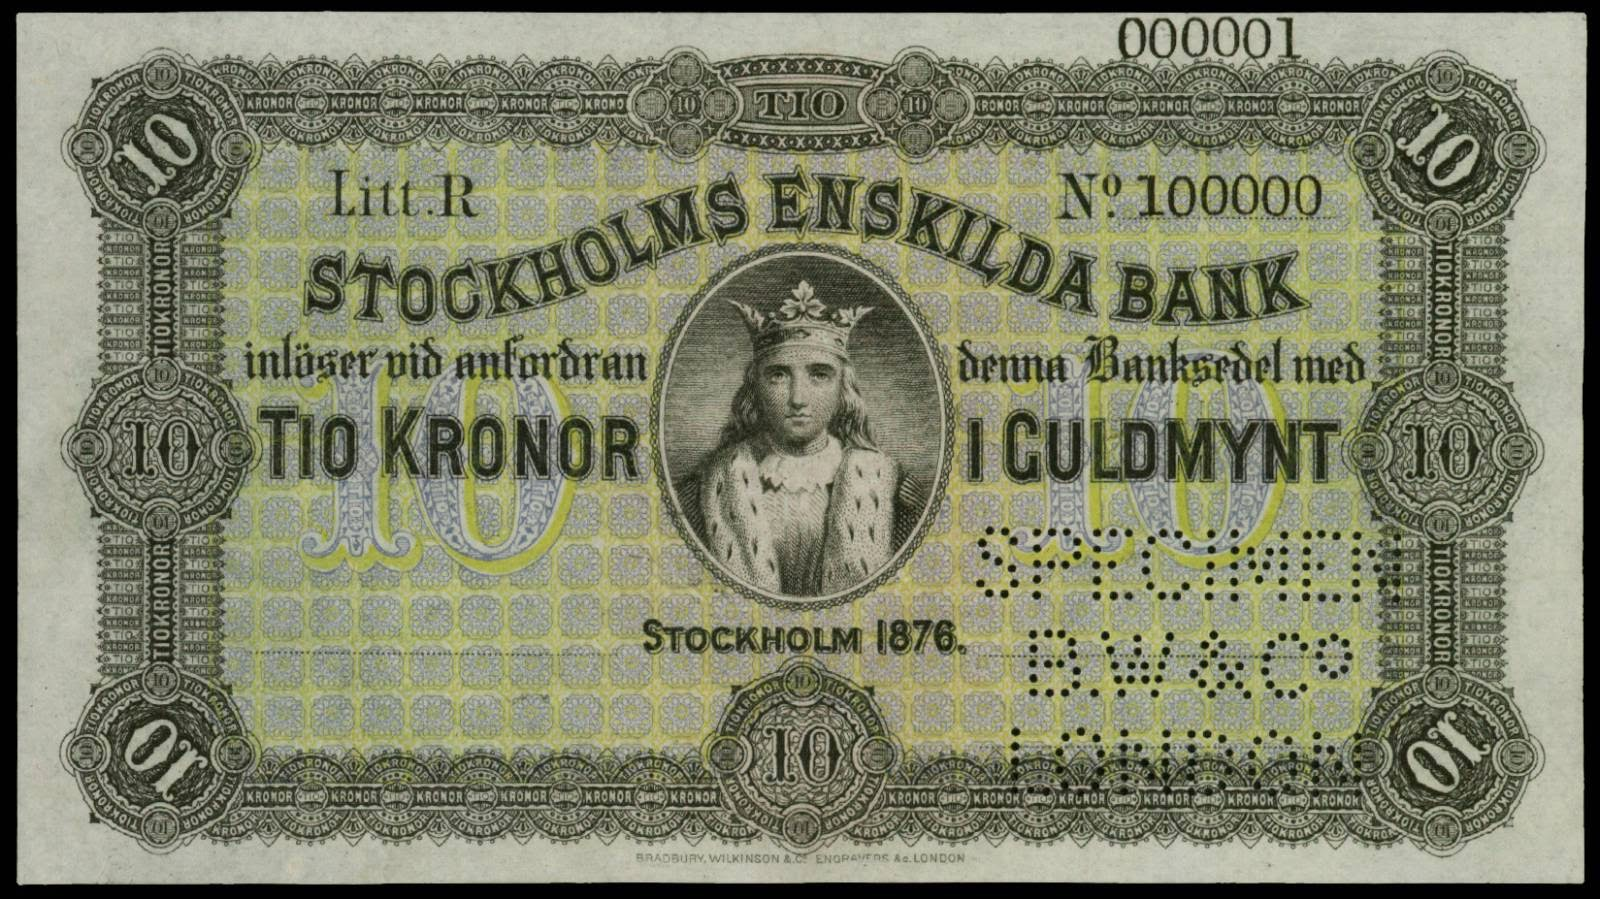
\includegraphics[width=7cm]{external/PrivateBankNoteStockholmEnskildaBank1876.JPG}
	\caption{\textit{The private bank 'Stockholms Enskilda Bank'(SEB) issued bearer
	promissory note. It promises to pay 10 crowns to the bearer upon demand in gold. 
	The exchange rate as per the Scandinavian Convention(Sweden, Denmark 27 may 1873, Norway 1 april 1877)\cite{nordic:crown}
	was 1 kilogram gold per 2480 crowns or 1 crown per 0.403g gold\cite{crown:gold}. 
 }}
	\label{fig:seb:promissory:note}
\end{figure}

By the late 19th century almost all major currencies was under the gold standard as seen in table \ref{tab:gold:standard}.

\begin{table}[!htb]
	\begin{tabular}{lllll}
		Nation & Currency & Period & Years \\
		France & Franc & 1814-1914 & 100 \\
		Netherlands & Guilder & 1816-1914 & 98 \\
		G.Britain & P. Sterling & 1821-1914 & 93 \\
		Switzerland & Franc & 1850-1936 & 86 \\
		Belgium & Franc & 1832-1914 & 82 \\
		Sweden & Kronor & 1873-1931 & 58 \\
		Germany & Mark & 1875-1914 & 39 \\
		Italy & Lira & 1883-1914 & 31 \\   
	\end{tabular}

	\caption{\textit{ Major European nations periods under the gold standard
			as composed by Ferdinand Lips\cite{lips:gold:wars} from 1975 Pickís Currency Yearbook data.
	}}
	\label{tab:gold:standard}
\end{table}

\subsection{Bank runs}

The introduction of the promissory note solved the two previously mentioned problems but also 
introduced trust.\footnote{Note that this a much wider problem than for only promissory notes. This trust model is what makes banks in the first place.} 

Although the gold deposits could be regularly audited by a third party there is little to no guarantee that the bank in question wouldn't issue more notes than gold it holds in reserve. Banks utilizing this sort of practice could go on for a very long time before getting caught. Consider a bank that issue twice as many notes as it holds gold in reserve. It would require 50\% of it's notes to be demanded before the bank would default.  
  
There has been many so called bank runs in history. The public gets suspicious about the bank and the trust disappears - leading to massive withdrawals in a short time span. Even if a bank is technically solvent, having assets tied up in different ventures, they could fail to deliver on the notes promises. This can also be viewed as a negative spiral, people start to withdraw, increasing the risk of default, more people start to withdraw due to the new higher risk. R.H. Patterson elaborates in detail the bank run in Great Britain in 1866 leading to the default of Overend, Gurney and Company and the behavior under panic: 

\begin{displayquote}
	"When a Panic occurs, a much more serious home-drain is produced upon the bank. At such time cheques fall somewhat into disrepute, so that merchants in some cases require payment in cash. The public also, to some extent, take to hoarding[...]. But a very large part of the drain upon the Bank of England in the form of hoarding ,[...],is made by other banks: for these banks being liable to unusual demands on the part of their customers, have to keep in hand a larger stock of money than usual"\cite{patterson:monetary:drains}
\end{displayquote}

Overall most larger institutions stayed solvent and bank runs is more an exception than a rule during this time period. Since all major currencies were denominated in gold the threshold for global trade sank. During the gold standard era the economy boomed with trade and is often known under the French term 'La Belle Epoque' or 'Beautiful era'. 

\onecolumn

\section{Elasticity of money}

It all came crashing down with the outbreak of the first world war. Nations central banks began to issue more notes than gold in reserve to fund the war effort. It effectively ended the gold standard and countries not affected by the war followed shortly after.

As response the Great Depression U.S President Franklin Roosevelt issued Executive order 6102 confiscating all gold coins, bullion and certificates and banned trade in gold\cite{roosevelt:6102}. The U.S Dollar was devalued the following year from \$20.67 per troy ounce to \$35 under the Gold Reserve Act\cite{gold:reserve:act} to enable spending their way out of recession. 

A new economic era began following ideas of Maynard Keynes of economic interventionism and monetary policies set to aid growth. Keynes rebutted the classical idea that 'supply creates its own demand' and that aggregated demand and aggregated supply may get stuck in an equilibrium with high unemployment\cite{keynes:general:theory}. This would motivate government intervention to increase the aggregated demand. While demand can be altered by a government in multiple ways the far most effective one was altering the money supply\footnote{The increased supply can be used directly by government but is usually used by lowering the funds rate, increasing investments and thus demand. Quantitative easing is another term describing this }. Although the dollar was still technically redeemable for gold the elastic money supply made it possible to steer the economy by means of monetary policy. 

The dollar was re-pegged multiple times between 1968-1971 as part of the Nixon chock\cite{bordo:bretton:woods}. In 1971 Nixon ended the Bretton Woods agreement\cite{bordo:bretton:woods}, the international agreement of exchange rates between currencies, rendering the dollar and all currencies pegged to the Dollar true fiat currencies. After the initial shock the free floating currencies failed to keep pace with gold due to money supply increase causing inflation(Se figure \ref{fig:gold:price:major:currency}).

\begin{figure}[!htb]
	\centering
	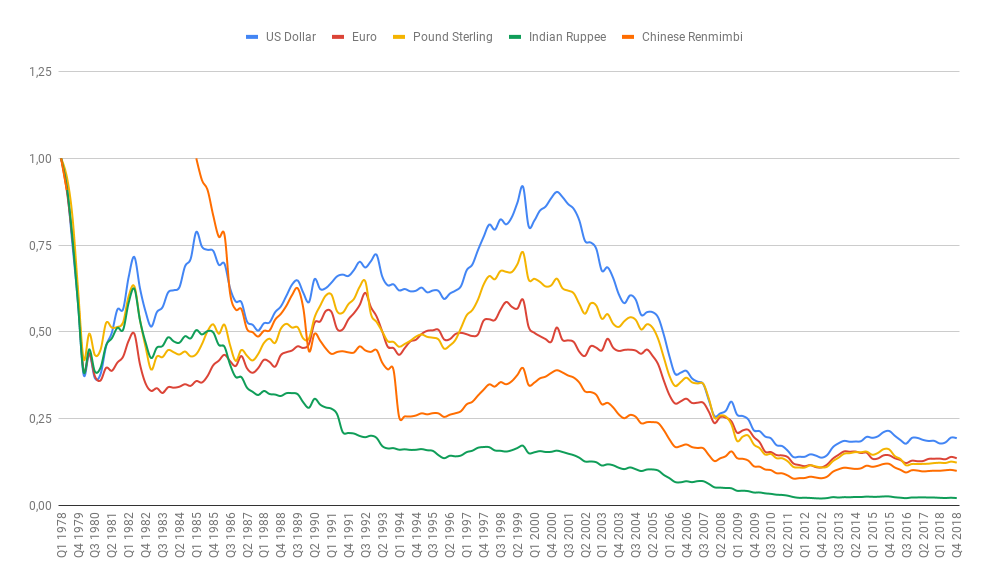
\includegraphics[width=16cm]{external/gold-price.png}
	\caption{\textit{The relation of major currencies against its value in gold since the end of the Bretton Woods agreement to
			today. The graph is composed with data from the World Gold Council\cite{world:gold:council}. 
	}}
	\label{fig:gold:price:major:currency}
\end{figure}

\twocolumn

\begin{table}[!htb]
	\begin{tabular}{llllll}
		Nation & Currency & Period & Highest monthly Inf. & Avg. daily Inf. & Type of index\\
		Hungary & Pengő & Aug. 1945 - Jul. 1946 & $ 4.19 × 10^{16}\% $ & 207\% & Consumer \\
		Zimbabwe & Dollar & Mar.2007 - Mid-Nov.2008 & $7.96 × 10^{10}\%$ & 98.0\% & Implied Exchange \\
		Yugoslavia & Dinar & 3 Apr.1992 - Jan.1994 & 313,000,000\% & 64.6\% & Consumer \\
		Germany & Papiermark & Aug. 1922 - Dec.1923 & 29,500\% & 20.9\% & Wholesale \\
		China & Yuan & Oct.1947 - Mid-May.1949 & 5,070\% & 14.1\% &	Wholesale \\
		Venezuela(§) & Bolívar & Jan. 2018 - ongoing & - & 4.1\% & - \\ 

	\end{tabular}
	\captionsetup{width=11cm}
	\caption{\textit{ Hyperinflation of selected fiat currencies. From the Hanke-Krus Hyperinflation Table \cite{hanke:krus:hyperinflation:table}. §The Venezuela numbers are only a projection by the International Monetary Fund
			and the dates and rate will most likely change with more accurate data\cite{hanke:hyperinflation} and when the inflationary period is over.
	}}
	\label{tab:inflation}
\end{table}

\subsection{Hyperinflation}

The major currencies seen in figure \ref{fig:gold:price:major:currency} is very far from worst in their ability to hold value. Fiat currencies are highly dependent on it's authority and their willingness to increase the money supply and history supplies us with some catastrophes as seen in table \ref{tab:inflation}.

During the last 250 years hyperinflation\footnote{There is no official definition of what constitutes hyper inflation but a rule of thumb seem to be over 50\% annual inflation.} have occured at least 54 times\cite{hanke:krus:hyperinflation:table}\cite{hanke:hyperinflation}. Many countries going through multiple inflationary periods, e.g. China 43-45, 47-49 and Georgia 92, 93-94. Hyperinflation devastates all savings and effectually letting savings subsidize the newly printed currency. The inflation narrows the time horizon of trade, since capital will go worthless in a short while, making it very difficult to formalize any long term investment or running a normal economy. 

\section{Trust}

The economic system built upon fiat currencies are based on the trust in the issuing body not to increase the money supply excessively. It's almost been common knowledge that value is lost in currencies, moving money away from currency and bonds into stock and real estate. Modern currencies have been decoupled from the underlying reasons of its nascence( see section \ref{sec:characteristics:money}) leading up to the failures of 08 coinciding with Nakamoto's publication completing full circle.

\newpage
\noindent
\vspace{6cm}

\subsection{Relevancy}
In many ways it helps to think of bitcoin as both a bearer instrument and as a monetary policy and how the system is designed as such. This section is an incomplete view on it's own and for further reading these recommendations are good starting points: 

\begin{itemize}
	\item Nick Szabo's blog Enumerated and above cited Shelling out\cite{szabo:shelling:out}\cite{szabo:unenumerated}.
	\item Saifedean Ammous's The bitcoin standard.\cite{ammous:bitcoin:standard}
	\item Waren Weber's paper A bitcoin standard.\cite{weber:bitcoin:standard}
\end{itemize}